\documentclass[preprint]{aastex}
\usepackage{graphicx}   % Including figure files
\usepackage{amsmath}    % Advanced maths comm
\usepackage{color,verbatim,url}
\usepackage{tabularx}
\usepackage[table,usenames,dvipsnames]{xcolor}\usepackage{pdflscape}
\usepackage{lastpage}

\definecolor{pink}{rgb}{0.858, 0.188, 0.478}
\definecolor{purple}{RGB}{76, 0,153}

\newcommand{\red}[1]{{\color{red}{#1}}}
\newcommand{\green}[1]{{\color{green}{#1}}}
\newcommand{\blue}[1]{{\color{blue}{#1}}}
\newcommand{\x}{\vec{x}}
\renewcommand{\d}[0]{{\rm d}}

\newcommand{\be}{\begin{equation}}  \newcommand{\ee}{\end{equation}}
\newcommand{\mb}[1]{\mbox{ #1 }}  
\newcommand{\ba}{\begin{eqnarray}}\newcommand{\ea}{\end{eqnarray}}
\newcommand{\bm}[1]{\mbox{\boldmath{$#1$}}}   %this is bold italic for MNRAS
\newcommand{\mat}[1]{\mathbfss{#1}}

\begin{document}

\title{\huge{Comment on `The Limits of Cosmic Shear'}}

\author{Members of the KiDS, CFHTLenS and RCSLenS collaborations\altaffilmark{1} ....}
%\email{tbd@tbd}

%\altaffiltext{1}{}

\begin{abstract}
Kitching et al. (2016) examine the impact of the flat-sky and Limber approximations that can be used when constraining cosmological parameters from the measurement of weak gravitational lensing by large-scale structures, also known as cosmic shear.  We support the core message of this paper that the use of such approximations should be considered in the future analysis of high precision surveys such as Euclid, LSST and WFIRST.  In this comment, we argue that these approximations have negligible impact for current surveys and are not able to explain away the tension between the constraints from some current weak lensing surveys and Planck.  Reducing uncertainty and characterising bias in photometric redshift estimation a critical task for the success of current and future surveys.  We highlight that sophisticated treatments of these uncertainties have already been explored in the literature and have been shown not to resolve the tension with Planck, in contrast to the message that Kitching et al. (2016) convey.

\end{abstract}
\section{Introduction}

The measurement of weak gravitational lensing by large scale structures provides a powerful cosmological probe of dark matter, dark energy and modifications to gravity.  As such it is the primary science goal of several current (KiDS, HSC, DES) and future (Euclid, LSST, WFIRST) large-scale surveys.   Interest in the results from these surveys is high as statistically significant deviations have been found between the cosmological parameter constraints from the CMB Planck experiment \citep{planck/cosmo:2015} in comparison to weak lensing constraints from both the Kilo-Degree Survey \citep[KiDS;][]{hildebrandt/etal:2016} and the Canada-France-Hawaii Telescope Lensing Survey \citep[CFHTLenS;][] {joudaki/etal:2016}.  If the source of this tension is not a result of so-far unconsidered sources of systematic errors in one or all experiments, extensions to the standard flat $\Lambda$CDM cosmological need to be considered.  \citet{joudaki/etal:2017} have shown, for example, that the tension can be resolved with an evolving dark energy model.

In this comment paper we discuss the flat sky and Limber approximations that can be used when deriving theoretical predictions for the principally used cosmic shear statistic, $\xi_\pm$, the two-point shear correlation function.   The Limber approximation for cosmic shear has been previously explored by \citet{giannantonio/etal:2012} finding that it provided sufficient accuracy for future cosmic shear studies.  Recently, however, \citet{kitching/etal:2016} reported that when considering the flat sky and Limber approximations in concert, tensions between weak lensing and CMB experiments can be reduced.  This was demonstrated with a re-analysis of the non-tomographic weak lensing data from the CFHTLenS survey \citep{kilbinger/etal:2013}.    

This comment is structured as follows.  In section~\ref{sec:theory} we clarify which brand of approximations, highlighted by \citet{kitching/etal:2016}, have been used in recent weak lensing analyses \citep{joudaki/etal:2016, hildebrandt/etal:2016, joudaki/etal:2017}.  We show that we are unable to replicate key results from \citet{kitching/etal:2016} and therefore do not expect these approximations to impact on the cosmological analysis of current surveys.    In section~\ref{sec:cfhtlens} we compare the `one-parameter' cosmological re-analysis of \citet{kitching/etal:2016} with the full six-parameter analysis by \citet{kilbinger/etal:2013}, arguing that this particular non-tomographic data set is not in significant tension with Planck.  We also briefly review the literature that has advanced our understanding since the original CFHTLenS analyses were published.   

In section~\ref{sec:photoz} we review our current knowledge of photometric redshift uncertainties and the sophisticated mitigation strategies that have already been applied to data.  We suggest that a possible misinterpretation in the direction of the redshift biases reported in \citet{choi/etal:2016} has lead to the incorrect conclusion of \citet{kitching/etal:2016} that these redshift biases can resolve the tension with Planck.  

\section{Theory}
\label{sec:theory}
\subsection{The Flat-Sky approximation and Extended Limber Approximation}
The baseline measurement for many cosmic shear studies has focused on the two-point shear correlation function between two tomographic bins $ij$ \citep[for more details see][and references therein]{miraldaescude:1991, kaiser:1992, bartelmann/schneider:2001}, given by
\be
\xi_\pm^{ij}(\theta) = \frac{1}{2\pi}\int_0^\infty \d\ell \,\ell \,P^{ij}_\gamma(\ell) \, J_{0,4}(\ell \theta) \, , 
\label{eqn:xiGG}
\ee
where $J_{0,4} (\ell \theta)$ is the zeroth (for $\xi_+$) or fourth (for $\xi_- $) order Bessel function of the first kind and $P_\gamma(\ell)$ is the shear power spectrum at angular wave number $\ell$ which can be related to the underlying matter power spectrum $P_\delta$, using a Limber approximation \citep{limber:1953} as,
\be 
P^{ij}_\gamma(\ell) = T_l \int_0^{\chi_{\rm H}} \d \chi \, \frac{q_i(\chi)q_j(\chi)}{[f_K(\chi)]^2} \, P_\delta \left( \frac{\nu(\ell)}{f_K(\chi)},\chi \right).
\label{eqn:Pkappa} 
\ee
Here $f_K(\chi)$ is the comoving angular diameter distance out to comoving radial distance $\chi$ and $\chi_{\rm H}$ is the comoving horizon distance.   The lensing efficiency function $q(\chi)$ is given in equation (5) of \citet{hildebrandt/etal:2016}, and the value of $\nu(\ell)$ depends on whether a baseline Limber approximation, $\nu(\ell) = \ell$, or the more accurate extended Limber approximation, $\nu(\ell) = \ell + 0.5$, from \citet{loverde/afshordi:2008} is used.   \citet{kitching/etal:2016} show that the pre-factor $T_\ell$ for the shear power spectrum is given by
\be
T_\ell = \frac{(\ell+2)(\ell+1)\ell(\ell-1)}{(\ell + 0.5)^4} = 1-{5\over 2\ell^2} +{\cal O}(\ell^{-3}) \, .
\label{eqn:Tl}
\ee
The corresponding pre-factor for the convergence power spectrum, along with the pre-factors for a range of other statistics such as the CMB lensing power spectrum and galaxy-galaxy lensing power spectrum, is given in \citet{jk12}.

When a survey is sufficiently small, a flat-sky approximation can be made reducing $T_\ell =1$ and $\nu(\ell) = \ell$.  In \citet{kitching/etal:2016} it is not fully clear which combinations of  $T_\ell$ and $\nu(\ell)$ are considered, so we review them all as summarised in Table~\ref{tab:Tl_nu}, also highlighting which combinations were used in recent cosmic shear analyses.

 \begin{table}[htb]
\begin{center}
\begin{tabular}{ | l | l | c | c  | c |}
\hline
Case & ID & $T_\ell$ & $\nu(\ell)$ & Used in \\ \hline
\citet{kitching/etal:2016} `Standard' & KSt & $1$ & $\ell$ & pre-2014 CFHTLenS papers \\
Baseline Limber `Flat' Sky &  LF & $\ell^4 / (\ell + 0.5)^4$ & $\ell$ & \\
Baseline Limber Spherical & LS & equation~\ref{eqn:Tl} & $\ell$ & \\
Extended Limber `Flat' Sky & ELF & $\ell^4 / (\ell + 0.5)^4$ & $\ell + 0.5$ & \\
Extended Limber Spherical & ELS & equation~\ref{eqn:Tl}& $\ell + 0.5$  & \\
Extended Standard Flat Sky & ESt & $1$ & $\ell + 0.5$ & \citet{joudaki/etal:2016} \&  \\
  &  & & & \citet{hildebrandt/etal:2016}$^*$\\\hline
 \end{tabular}
 \end{center}
 \caption{\label{tab:Tl_nu}Variations on the different approximations that can be made when calculating the shear power spectrum $P_\gamma(\ell)$ (equation~\ref{eqn:Pkappa}), using a Limber approximation.  $^*$We confirm that there is a typographical error in equation 4 of \citet{hildebrandt/etal:2016} which should include the extra term of `$+0.5$' in $\nu(\ell)$ that was incorporated in the cosmological analysis.} 
 \end{table}

Figure~\ref{fig:Cl_xi} shows theoretical models for the shear power spectrum $P_\gamma(\ell)$ (equation~\ref{eqn:Pkappa}), and the shear correlation function (equation~\ref{eqn:xiGG}) for the different variations on the approximations listed in Table~\ref{tab:Tl_nu}.   The Standard and Spherical models agree at the few percent level above $\ell>10$ and below $\theta< 100$ arcmin.  The two outliers are the Baseline and Extended `Flat' Sky Limber cases (LF and ELF) where the \citet{kitching/etal:2016} `Flat' Sky approximation has been made with
\be
T_\ell^{\rm `Flat'} = \ell^4 / (\ell + 0.5)^4 = 1-{2\over \ell}+{5\over 2\ell^2} +{\cal O}(\ell^{-3}) \, . 
\ee    
We argue that applying the approximation, that $\ell \pm x \approx \ell$, where $x$ is small, only to the numerator of equation~\ref{eqn:Tl} is inconsistent.  By comparing the expansions of equations~\ref{eqn:Tl} and~\ref{eqn:Tlflat}, we see that the \citet{kitching/etal:2016} `Flat' Sky approximation effectively introduces a new term $2/\ell$ making it more deviant from the full spherical solution in comparison to the standard $T_\ell = 1$ case.    To our knowledge, this form of the flat-sky approximation has not been used in cosmic shear studies to date.  

As shown in the lower panels of Figure~\ref{fig:Cl_xi}, the `standard flat' sky approximation used by recent cosmic shear surveys\footnote{The KSt approximation was used for pre-2014 CFHTLenS analysis and the ESt approximation was used for recent CFHTLenS and KiDS analyses}, where $T_\ell = 1$, recovers a very similar result to the spherical sky case.  Over angular scales used in the recent KiDS cosmic shear analysis (where the maximum angular scale $\theta<50.7$ arcmin is shown dashed), these curves differ by less than 1\%.  As such the standard flat-sky approximations that have been used will not impact the cosmological analyses of current surveys.
 
 \begin{figure}
 \begin{center}
 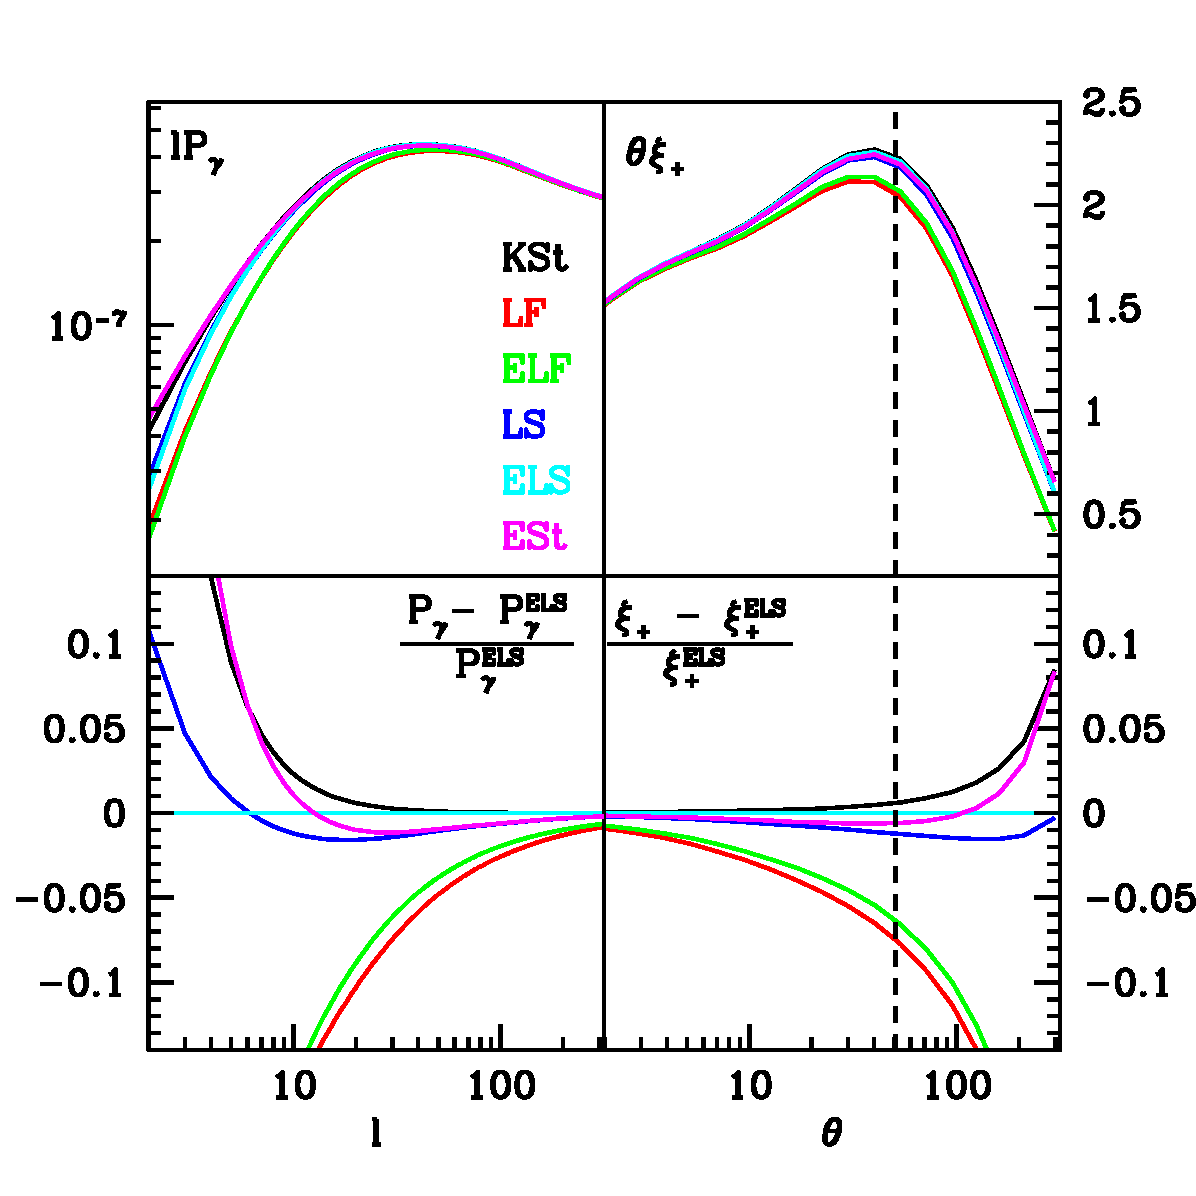
\includegraphics[width=0.85\textwidth]{figures/Cl_xi_comp.pdf}
 \caption{ \label{fig:Cl_xi}\emph{Upper Panels:} Theoretical models for the shear power spectrum (\emph{left}) and shear correlation function $\xi_+$ (\emph{right}) for the different approximations listed in Table~\ref{tab:Tl_nu}, assuming a \citet{planck/cosmo:2015} cosmology and the 2D CFHTLenS redshift distribution. \emph{Lower Panels:} Deviations with respect to the extended Limber spherical sky model (ELS).    The dashed lines in the right panels show the largest angular scale used in the recent KIDS cosmic shear analysis where an Extended Standard (ESt) analysis was used.}
 \end{center}
 \end{figure}
 
 \subsection{Cosmic shear without the Limber Approximation}
In collecting our comments on \citet{kitching/etal:2016} we contacted colleagues who had previously tested the impact of the Limber approximation on cosmic shear studies by comparing a Limber-approximated cosmic shear power spectrum with an exact calculation.  The majority of these analyses, carried out many years ago, remained unpublished in peer reviewed journals as no significant deviation was found\footnote{See for example appendix M of the 2010 PhD thesis from Donghui Jeong (\url{http://www.personal.psu.edu/duj13/dissertation/djeong_diss_appM.pdf}) and Chapter 7 of 2012 PhD thesis from Nicolas Van de Rijt (\url{http://ipht.cea.fr/Docspht/articles/t12/080/public/these_vanderijt2012.pdf}).}.  One notable exception, however, is \citet{giannantonio/etal:2012} who find that for a cosmic shear power spectrum, the extended Limber approximation is consistent with the exact calculation for $\ell>5$, with any differences well within cosmic-variance errors for a Euclid-like survey\footnote{\citet{kitching/etal:2016} comment on this result, but indicate that it is in error owing to the application of a fixed low-$\ell$ limit.  \citet{giannantonio/etal:2012} however state that this limit is only applied in a positive curvature case.}.  They conclude that the Limber approximation works so well for cosmic shear owing to the wide redshift distribution of the lensed sources.  This is in comparison to the case of galaxy power spectra,  where narrower redshift bins result in a significant difference between the Limber and non-Limber cases \citep[see also][]{simon/2007}.   Given this body of work, we argue that the assertion by \citet{kitching/etal:2016} that the majority of cosmic shear data analyses to date have made an `axiomatic assumption (i.e. an unquestioned and untested assumption at the beginning of the analysis)'  is unwarranted.  Not only is there published work that has questioned and tested the Limber approximation for the cosmic shear power spectrum, individual teams have also verified this result internally for their own cosmic shear analyses.    

Given the insignificant effect of using the Limber approximation found by various groups, the ability to calculate an exact non-Limber solution has unfortunately not been maintained in many theoretical codes over the years.  Instead these codes have evolved to account for critical approximations such as the impact of baryon feedback on the matter power spectrum and non-zero neutrino masses \citep[see for example][]{joudaki/etal:2016, mead/etal:2016}.    Two exceptions to this are recent updates to CLASS \citep{blas/lesgourgues/tram:2011,audren/etal:2013} and CosmicFish \citep{raveri/etal:2016}.  On-going code comparisons have, however, revealed differences that are larger than the expected impact of Limber or non-Limber approximation.   We are therefore unable to readily determine non-Limber theoretical calculations for the shear-correlation function to directly compare with the results of \citet{kitching/etal:2016}.   Instead we refer the reader to Figure 3 of \citet{giannantonio/etal:2012} to draw their own conclusions about the impact of this effect.



 
 
 
 
 
 
 

\section{Advances in understanding since CFHTLenS}
\label{sec:cfhtlens}
The Canada-France-Hawaii Telescope Lensing Survey (CFHTLenS) represented a major step forward for the field of weak gravitational lensing, in terms of improved accuracy in data reduction \citep{erben/etal:2013}, the implementation of PSF-Gaussianised matched multi-band photometry \citep{hildebrandt/etal:2012}, cross-correlation clustering analysis between photometric redshift slices to verify tomographic redshift distributions \citep{benjamin/etal:2013}, accurate calibrated shape measurements \citep{miller/etal:2013} and a full suite of informative systematic tests to select a clean data set \citep{heymans/etal:2012}.    Since the public release of this survey in 2013, the community has continued to scrutinise and advance our understanding of CFHTLenS by identifying a number of areas where analyses could improve:
\begin{itemize}
 \item{\citet{choi/etal:2016} identified biases in the tomographic photometric redshift distributions using a more effective clustering analysis, in comparison to \citet{benjamin/etal:2013}, by incorporating newly overlapping spectroscopy from the Sloan Digital Sky Survey.  The CFHTLenS tomographic cosmological analysis was then revisited by \citet{joudaki/etal:2016} in order to include a full redshift error analysis based on the results from \citet{choi/etal:2016}, discussed further in section~\ref{sec:photoz}.}
\item{\citet{asgari/etal:2016} used the stringent `COSEBI' statistic to identify significant non-lensing `B-mode' distortions when the CFHTLenS data was split into tomographic slices.}
\item{\citet{kuijken/etal:2015} showed that the CFHTLenS shear calibration corrections derived in \citet{miller/etal:2013} were underestimated as a result of an imperfect match between the galaxy populations in the data and image simulations.}
\item{\citet{fenechconti/etal:2016} demonstrated that the CFHTLenS data would have been subject to a weight bias that favours galaxies that are more intrinsically oriented with the point-spread function.  They also showed that the impact of calibration selection biases, that were not considered in \citet{miller/etal:2013}, would have lead to the over-correction of multiplicative shear bias in the CFHTLenS analyses, by a few percent.}
\item{\citet{joudaki/etal:2016} updated the CFHTLenS covariance matrices using larger-box numerical simulations that were less subject to the lack of power on large scales.}
\end{itemize}
All these advances in our understanding were incorporated and accounted for in the recent KiDS cosmic shear analysis \citep{hildebrandt/etal:2016} which reports a $2.3 \sigma$ tension with Planck.  Efforts are now underway to fully re-analyse CFHTLenS using the advanced KiDS analysis pipeline with revised shape measurements and calibrations for the shear and photometric redshifts.  Until this analysis is complete we note that these known shortcomings with the original CFHTLenS results impact in different ways on the cosmological conclusions that one can draw from the survey.

The \citet{kitching/etal:2016} re-analysis of the 2D CFHTLenS data from \citet{kilbinger/etal:2013} chose to only vary $\sigma_8$ in their analysis, fixing all other parameters to Planck values. They find a conditional value of $\sigma_8 = 0.789 \pm 0.015$ for their `standard' analysis (row 1 in Table~\ref{tab:Tl_nu}). This result can be compared to the full five-parameter fit from \citet{kilbinger/etal:2013} who find $S_8=\sigma_8(\Omega_m/0.3)^{0.6} = 0.74 \pm 0.03$.   We argue that this reduction in the relevant error by a factor of $\sim 2$, could easily mislead, making it appear that the impact of removing all approximations from the theoretical analysis is more significant for current surveys than it is in reality.  Nevertheless, we repeated the `one-parameter' analysis for the range of Limber-approximated cases listed in Table~\ref{tab:Tl_nu} and are unable to confirm the results quoted by \citet{kitching/etal:2016}.   We find the lowest conditional value of $\sigma_8 = 0.746 \pm 0.023$ for the `Standard' (KSt) case and the highest conditional value of $\sigma_8 = 0.749 \pm 0.023$ for the `Extended Limber Flat' (ELF) case, a maximum change of $\Delta \sigma_8 = 0.0026 = 0.11 \sigma$.  These findings are in disagreement with \citet{kitching/etal:2016} who find a shift of $\Delta \sigma_8 = 0.007 = 0.5\sigma$ between their `standard' analysis (row 1 in Table~\ref{tab:Tl_nu}) and their `Limber' analysis (which we believe corresponds to the Extended Limber spherical (ELS) case in Table~\ref{tab:Tl_nu}).  

The most relevant case to consider is differences between the fiducially used `Extended Standard Flat' (ESt) case with the preferred `Extended Limber Spherical' (ELS) case.  Here we find that the constraints are identical at the $0.01\sigma$ level.  As expected from the comparison in Figure~\ref{fig:Cl_xi}, and given the low signal-to-noise CFHTLenS measurements on large scales, we conclude that the different combinations of assuming flat or spherical sky, baseline or extended Limber, make little difference to the cosmological parameter constraints, even in a `one-parameter' analysis.    

We note that \citet{kitching/etal:2016} use their `Flat' approximation for their `Full' non-Limber analysis of the CFHTLenS data.   This is because on a sphere, correlation functions cannot be related to the power spectrum by a Hankel transform (e.g. equation~\ref{eqn:xiGG}) as the power spectrum is not defined for non-integer $\ell$.   In Figure~\ref{fig:Cl_xi}, however, we show that this chosen version of a flat-sky approximation serves to exacerbate the tension in theoretical models when a flat-sky solution is compared with the spherical-sky solution in the Limber approximated case.  This is not the case when considering the standard $T_\ell = 1$ flat-sky approximation that has been used in the majority of cosmic shear studies to date.  We would therefore argue that it is more appropriate to use a $T_\ell = 1$ flat-sky approximation when carrying out a `Full' non-Limber analysis of the shear correlation function obtained from the Hankel transformation (equation~\ref{eqn:xiGG}).

\subsection{Comparison of two-point shear statistics; the two-point correlation function, mass aperture statistic and COSEBIs}
\citet{kilbinger/etal:2013} present a detailed comparison of cosmological constraints obtained from a range of different two-point shear statistics including the shear correlation function, $\xi_\pm$, the aperture-mass dispersion, $\langle M_ {\rm ap} \rangle ^2$ \citep{schneider/etal:1998}, and the COSEBIs, $E_n$ \citep{schneider/etal:2010}.  These statistics are linearly related to the power spectrum via integrals of the form,
%
\begin{align}
\label{eqn:integ}
& E_n =\int_0^{\infty}\frac{\d \ell \ell}{2\pi} W_n(\ell) P(\ell)\;,\\ \nonumber
& \langle M_ {\rm ap} \rangle ^2(\theta)=\int_0^{\infty}\frac{\d \ell \ell}{2\pi} U^2_\theta(\ell) P(\ell)\;,
\end{align}
%
where $W_n(\ell)$ and $U^2_\theta(\ell)$ are defined in \cite{schneider/etal:2010} and \cite{schneider/etal:1998}. The corresponding equation for $\xi_\pm$ is given in equation~\ref{eqn:xiGG}.
Figure~\ref{fig:filters} shows the integrands of these statistics 
for two cases, normalised to their maximum value, where the integrands are of the form $\ell F(\ell) P(\ell)$. For $\xi_\pm$, $P(\ell)$ is equal to the sum of the E and B-mode power spectra, motivating the development of the aperture-mass dispersion statistic, $\langle M_ {\rm ap} \rangle ^2$.  This statistic is, however, a lossy conversion and is biased by small angular separations, where blending of galaxies makes shear measurement challenging \citep{kilbinger/etal:2006}.  The COSEBIs statistic tackles both these shortcomings.  The upper two panels of figure~\ref{fig:filters} show the integrands\footnote{Note that the lower left panel of Fig. 1 in \citet{kitching/etal:2016} shows an integrated form of this function for a maximum angular separation of $100'$. However, in \citet{kilbinger/etal:2013}, the data used in \citet{kitching/etal:2016}, $\theta$ is between $0.8'$ and $350'$.} of $\xi_\pm$ for $\theta=100'$ and $\theta=350'$. The lower middle panel in Figure~\ref{fig:filters} shows the COSEBIs integrands for two angular ranges, $[1',100']$ and $[0.8',350']$, where we only show the integrands for the lowest COSEBIs mode, $E_1$, as the higher modes generally probe larger $\ell$-modes.  Finally, the lowest panel shows the integrands of aperture mass dispersion statistics, for the same two maximum angular ranges. 

\begin{figure}[!htp]
\begin{center}
\begin{tabular}{ccc}
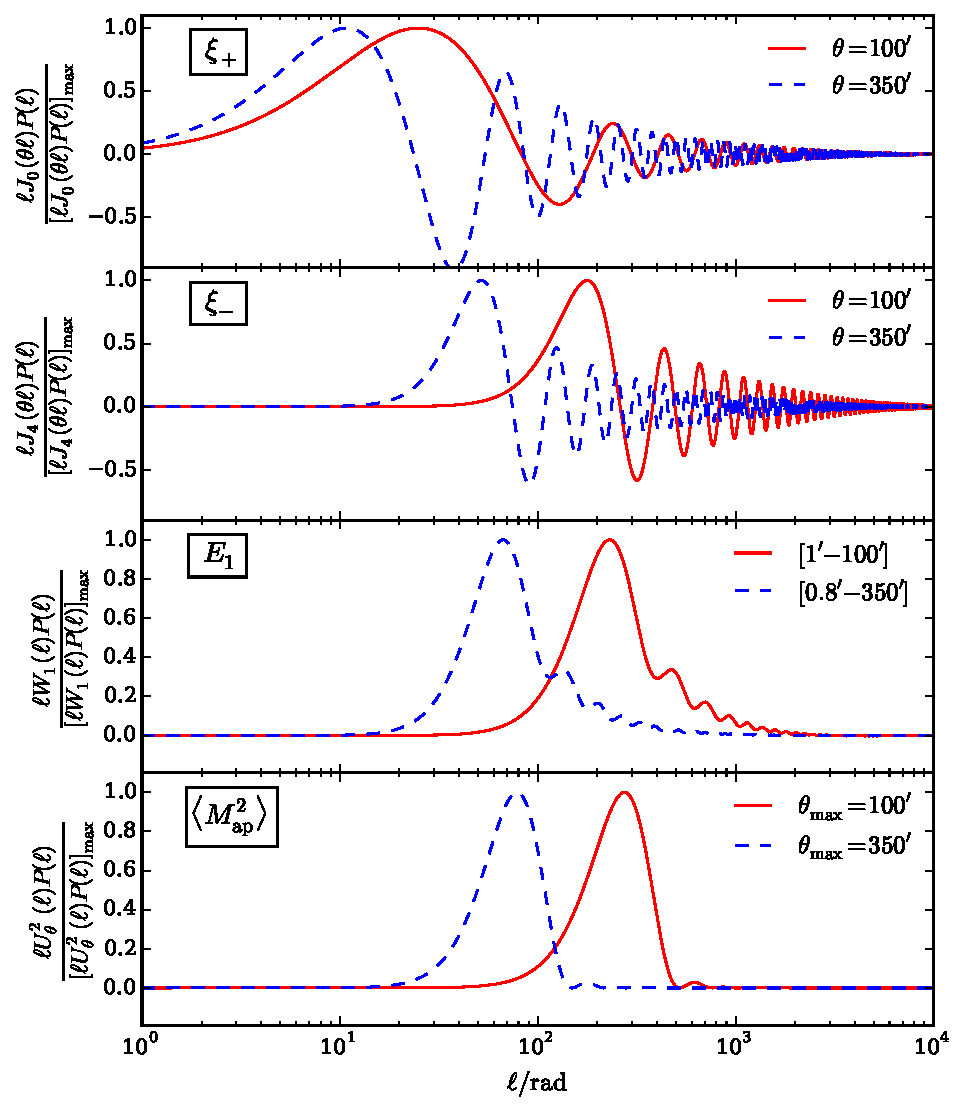
\includegraphics[width=\textwidth]{figures/IntegAll.pdf} \\
\end{tabular}
\caption{ \small{\label{fig:filters}. Integrand of $\xi_+$ (upper), $\xi_-$ (upper middle), $E_1$ (lower middle, E-COSEBIs) and $\langle M_{\rm ap} \rangle^2$ (lower panel).
All integrands are of the form $\ell F(\ell) P(\ell)$, where $F(\ell)$ is the corresponding weight-function
for each statistic and $P(\ell)$ is the E-mode convergence power spectrum, with the exception of $\xi_\pm$, for which
$P(\ell)$ is equal to the sum of the E and B-mode power spectra. 
Two cases are shown for each statistic as listed in each caption.
For the aperture mass statistic $\theta_{\rm max}=2\theta$ is shown. 
Note that higher order COSEBIs modes generally probe larger $\ell$-modes, 
hence here we only show the lowest mode $E_1$. All values are normalized with respect to their maximum value. }
}
\end{center}
\end{figure}

From Figure~\ref{fig:filters} we can see that the two-point cosmic shear statistics tested by \citet{kilbinger/etal:2013} exhibit different dependences between the angular scales sampled and the $\ell$-range probed.   
If a significant bias had been introduced at low-$\ell$ by using flat-sky and Limber approximations, we would then expect to see a systematic shift between the different two-point statistics with the COSEBIs statistic being essentially unaffected as it only includes modes with $\ell \gtrsim 20$.  This is found not to be the case with all three statistics finding $\sigma_8 (\Omega_m/0.27)^\alpha = 0.79$ with errors that range from $0.03$ to $0.06$ for the full five-parameter fit, and $\alpha$ ranging from $0.59$ to 0.7 \citep[see Table 5 of][]{kilbinger/etal:2013}.  This comparison further supports our argument that the approximations highlighted by \citet{kitching/etal:2016} have negligible impact for current surveys.


\subsection{On the Validation of Methods on Simulations}
It is discussed in \citet{kitching/etal:2016} that the validation of cosmic shear estimators on mock catalogues could also be affected by the approximations they investigate.  We agree that a full sky mock should be compared to a full curved sky non-Limber prediction.  It is then suggested, however, that the discrepancies already reported between existing mocks and the predictions could be attributed to these approximations, as opposed to a finite box effect \citep{kiessling/etal:2011, harnois-deraps/etal:2012, harnois-deraps/vanwaerbeke:2015}.  Going beyond flat-sky and Limber could improve the agreement, however this cannot explain the results of \citet{harnois-deraps/vanwaerbeke:2015} who demonstrate that the large-scale under-estimation of power varies with the simulation box size. This volume effect was verified by comparing the $\xi_+$ statistic at large angular scales between simulation volumes with box sides  ranging from $147\;\rm{Mpc/h}$ to $515\;\rm{Mpc/h}$ \citep[see Fig. 5 in][]{harnois-deraps/vanwaerbeke:2015}. The increase of power loss with decreasing box size was shown to be fully-modelled by excluding the super-box $k$-modes in the Limber predictions, something that the approximations discussed in \citet{kitching/etal:2016} would be unable to explain.

We note that any future comparison of mock data with full curved sky non-Limber predictions would place requirements on the input weak lensing simulations.  Many work with parallel plane mass-sheets as opposed to curved sky mass-sheets and at large angles these two approaches differ, regardless of the box size. 

\subsection{On the application to CMB lensing}
\citet{kitching/etal:2016} discuss how corrections to the Limber and flat-sky approximations would also affect predictions involving the shear and convergence cross-spectrum, such that the cross-correlation of CMB lensing and galaxy lensing should include a pre-factor $ [\ell(\ell+1)]^2/(\ell+ 0.5)^4 = 1-{1\over 2\ell^2}+{\cal O}(\ell^{-3})$.   We have verified that this term would have negligible impact on current measurements, given the relatively low signal to noise ratio.  For example, most measurements \citep{hand/etal:2015, liu/hill:2015, kirk/etal:2016,harnois-deraps/etal:2016} are carried over angular multipoles in the range $\ell \in [20-2000]$.  The size of the pre-factor, averaged over this range, is of the order of 0.01\%. In comparison, the size of the statistical error bars are of the order 25-35\% with additional uncertainty due to photometric redshifts (10-15\%) and intrinsic galaxy alignments (10-15\%). The pre-factor reaches 1\% only for $\ell < 7$, which may become relevant for very large upcoming surveys but is negligible for current surveys. 

\subsection{On the quadratic estimator of the cosmic shear power spectrum}

\citet{kitching/etal:2016} state that `the derivative of a Limber-approximated power spectrum is not equal to the Limber-approximation of the derivative'. Based on this statement they conclude that `statistics that use Limber-approximated quadratic estimators to measure the cosmic shear power spectrum are not accurate' and refer explicitly to the quadratic estimator implementation used in \citet{Koehlinger2016} to measure the cosmic shear power spectrum from CFHTLenS. In this quadratic estimator implementation, however, the Limber approximation does not enter. 

The quadratic estimator algorithm was originally presented by \citet{Hu2001} in the context of cosmic shear and has also been applied to other shear data sets (e.g. \citealt{Brown2003, Heymans2005, Lin2012}).   The aim of the method is to find the best-fitting power spectra assuming a Gaussian likelihood function $\mathcal{L}$. The likelihood depends on the shear data vector and its covariance $\mathbf{C}$ which consists of the sum of the shear correlation matrix $\mathbf{C}^\mathrm{sig}$ and the noise matrix $\mathbf{C}^\mathrm{noise}$. The shear correlation matrix can be written as a linear combination of piece-wise constant band powers $\mathcal{B}$ approximating the Fourier transforms of the shear correlations, i.e. their power spectra (cf. equations~3,~10 in \citealt{Koehlinger2016}). The best-fitting power spectra are found by iteratively stepping through a Newton--Raphson method in order to find the root of $\diff \mathcal{L}/ \diff \mathcal{B} = 0$ \citep{Bond1998, Seljak1998}. In the subsequent equations of the Newton--Raphson method only derivatives of the full covariance matrix enter, where the derivatives are taken with respect to band powers\footnote{i.e. $\partial \mathbf{C} / \partial \mathcal{B}_A$, where $A$ is a superindex over the type of the band, band-power bin and redshift correlation, see appendix\~A in \citealt{Koehlinger2016}.}.  We emphasize that the only approximation entering this algorithm is the flat-sky approximation when introducing the Fourier decomposition of the spin-2 shear field.    This approximation is appropriate and accurate for current surveys as $\ell>80$  in all analyses published to date.


\section{Photometric redshift bias and uncertainty}
\label{sec:photoz}
In \citet{choi/etal:2016} a cross-correlation clustering analysis, between photometric redshift slices and overlapping spectroscopic redshifts, is used to determine linear biases in the CFHTLenS photometric redshift distributions.   The maximum redshift $z_B<0.9$ in this analysis was limited by the redshift overlap with the spectroscopic sample\footnote{The implication of a $z_B < 0.9$ high-redshift limit is that the analysis is unable to constrain the high-redshift tails of the redshift distributions due to the lack of overlapping high-redshift spectroscopic samples. As such the results from \citet{choi/etal:2016} are only the first important step towards a detailed understanding of the CFHTLenS tomographic redshift distributions and as such may be revised in the future.}.  \citet{choi/etal:2016} found significant biases in the redshift distributions used in the original CFHTLenS analyses,
concluding that any re-analysis of CFHTLenS should include systematic error terms to account for bias and scatter.    This re-analysis was presented in \citet{joudaki/etal:2016} where the impact of correcting for the biases determined by \citet{choi/etal:2016}, including their associated errors, served to reduce the overall constraining power of the survey and hence also the tension between constraints.  The best-fit model, however moved further from the Planck-preferred model, in agreement with the `toy-model' analysis of \citet{choi/etal:2016} which concluded that the effect of these biases would be to {\it reduce} the recovered amplitude of $\sigma_8$ by $\sim 4$\%. 

\citet{choi/etal:2016} additionally showed that applying a simple linear shift to the photometric redshift distributions was insufficient when modelling the true underlying redshift distribution.  In \citet{hildebrandt/etal:2016}, a direct calibration method was used to determine the redshift distribution of four tomographic bins.  Multiple bootstrap samples of the resulting calibrated distribution allowed for the characterisation of both the uncertainty in the mean and shape of the redshift distribution.  The inclusion of this more sophisticated treatment of photometric redshift errors was not found to alleviate the tension between Planck and KiDS parameter constraints.

\cite{kitching/etal:2016} use a linear fit to the biases determined by \citet{choi/etal:2016} in order to extrapolate the results beyond the photometric redshift limit of $z_B<0.9$ and determine a bias at each redshift.  They then correct the non-tomographic \citet{kilbinger/etal:2013} redshift distribution with this bias relation.  They report that this correction results in an {\it increase} to the recovered amplitude of $\sigma_8$ by $\sim 4$\%, which resolves the tension with Planck.   We are unable to recover this conclusion using two different methods.   Based on the \cite{kitching/etal:2016} relation, the predicted shift at the mean CFHTLenS redshift $z=0.747$ is $\Delta_z = 0.056$, where we use the convention from \citet{choi/etal:2016} that a positive $\Delta_z$ serves to increase the true mean redshift.  Using the same relation to individually shift each component of the full \citet{kilbinger/etal:2013} redshift histogram also results in a change to the mean redshift of $\Delta_z = 0.056$.  Increasing the mean redshift implies a reduction in the recovered amplitude of $\sigma_8$.  Using the same `toy-model' analysis of \citet{choi/etal:2016} we would expect this change in the mean redshift to {\it reduce} the recovered amplitude of $\sigma_8$ by $\sim 5$\%.    From this we suggest that \cite{kitching/etal:2016} could have misinterpreted the direction of the redshift biases reported in \citet{choi/etal:2016}. 



 

\section{Conclusion}
\label{sec:conclusion}
In this comment we have highlighted a number of shortcomings in the analysis presented in \cite{kitching/etal:2016}.  We argue that the flat sky and Limber approximations that can be used in cosmic shear analyses are not able to explain away the tension between current weak lensing and Planck results, in contrast to the message that \cite{kitching/etal:2016} convey.  Our critique should not, however, detract from the important core message of their paper, that future surveys will need to consider these approximations and optimise their statistical analyses accordingly.  For example moving from the standard two-point shear correlation function statistic to the more stringent `COSEBI' statistic \citep{schneider/etal:2010} renders the cosmic shear measurement completely insensitive to the low-$\ell$ scales where these approximations become important.  


\bibliographystyle{apj}
\bibliography{Limber_Comment}
\end{document}
